%%-----------------------------------------------------------------------------
%% Technische Hochschule Ingolstadt 
%%
%% To be used as style template for a Bachelor's/Master's Thesis in the 
%% Faculty of Electrical Engineering and Information Technology
%%
%% by Prof. Dr.-Ing. Michael Mecking  
%%-----------------------------------------------------------------------------

\documentclass[11pt, titlepage, english, a4paper]{report}

\usepackage[top=1.2in, bottom=1.4in, inner=1.1in, outer=1.1in]{geometry}


\usepackage[utf8]{inputenc}         %% Support for UTF-8 input encoding
\usepackage[T1]{fontenc}            %% 8-bit font encoding... more glyphs... 
                                    %% easier copy & paste from the output PDF
\usepackage[english]{babel}         %% English document with English settings
\usepackage{titlesec}               %% change of appearance of chapters
\usepackage{fancyhdr,lipsum}        %% Control of headers and footers
\usepackage{lmodern}                %% Modern font family

\usepackage{tocbibind}              %% Ensures appendices, bibliograph appear in ToC
\usepackage{algorithmic}            %% Number of commands for typesetting popular algorithmic constructs
\usepackage{listings}               %% Typeset programming code within LaTeX
\usepackage{longtable}              %% Write tables that continue to the next page
\usepackage{float}                  %% Prevents repositioning of tables using [H]

\usepackage{amsmath,bm}             %% AMS math symbols and bold math
\usepackage{amsbsy}                 %% Bold mathematics symbols where appropriate fonts exist
\usepackage{amsfonts}               %% Additional mathematical fonts
\usepackage{amssymb}                %% Extra mathematical symbols
\usepackage{eulervm}                %% Don Knuth's beautiful (my favorite!) font
\usepackage{fixmath}                %% Uppercase Greek be typeset in italic style

\usepackage[pdftex]{graphicx}       %% Include graphics in PDF mode
\usepackage[pdftex]{xcolor}         %% Handle colors in PDF mode
\usepackage[autostyle]{csquotes}    %% Quotation according to language requirements
\usepackage{units}                  %% Proper spacing for units
\usepackage{hhline}                 %% More control over table border lines
\usepackage{titling}                %% Control over document title elements
\usepackage{blindtext}              %% Generate dummy text
\usepackage{multirow}               %% Multi-row cells in tables
\usepackage{lastpage}               %% Reference the last page of the document
\usepackage{afterpage}              %% Defer command execution to new page
\usepackage{hyperref}               %% Hypertext in LaTeX (clickable links)

\usepackage[toc, acronym]{glossaries} 			
\makeglossaries	

\usepackage[intoc]{nomencl}         %% uncomment if not used
\makenomenclature

%%-----------------------------------------------------------------------------
%%  TikZ setup
\usepackage{tikz}                   %% add more libraries if needed
\usetikzlibrary{arrows,automata,shadows,positioning,decorations.pathreplacing,%
    matrix,calc,backgrounds,patterns,shapes,shapes.gates.logic.IEC,%
    intersections,through}

%%-----------------------------------------------------------------------------
%%  some common abbreviations using better LaTeX formatting
\newcommand{\ie}{i.e., }
\newcommand{\eg}{e.g., }
\newcommand{\etc}{etc.\@ }

%%-----------------------------------------------------------------------------
%%  Definition of mathematical functions/operators for simpler syntax
\DeclareMathOperator{\sign}{sign}
\DeclareMathOperator{\Mod}{mod}
\DeclareMathOperator{\artanh}{artanh}
\DeclareMathOperator{\arcosh}{arcosh}
\DeclareMathOperator{\arc}{arc}
\DeclareMathOperator{\Arg}{Arg}
\renewcommand{\Re}{\mathrm{Re}}
\renewcommand{\Im}{\mathrm{Im}}
\DeclareMathOperator{\spn}{span}
\DeclareMathOperator{\defekt}{def}
\DeclareMathOperator{\diag}{diag}
\DeclareMathOperator{\grad}{grad}
\DeclareMathOperator{\argmin}{arg\,min}
\DeclareMathOperator{\argmax}{arg\,max}

%%-----------------------------------------------------------------------------
%%  use the provided LaTeX-style file for your seminar paper
%%-----------------------------------------------------------------------------
%% LaTeX style template for Bachelor/Master Thesis in the
%% Faculty of Electrical Engineering and Information Technology
%% by: Prof. Dr.-Ing. Michael Mecking, Technische Hochschule Ingolstadt
%%-----------------------------------------------------------------------------

\makeatletter
\def\cleardoublepage{\clearpage\if@twoside \ifodd\c@page\else
	\hbox{}
	\vspace*{\fill}
	\begin{center}
	\end{center}
	\vspace{\fill}
	\thispagestyle{empty}
	\newpage
	\if@twocolumn\hbox{}\newpage\fi\fi\fi}
\makeatother

\clearpage{\pagestyle{empty}\cleardoublepage}
\pagestyle{fancy}
\setlength{\headheight}{25pt}
\renewcommand{\sectionmark}[1]{\markright{\thesection.\ #1}}

%%-----------------------------------------------------------------------------
%% for better readbility
\linespread{1.3}

\makeatletter
\def\@subtitle{\@latex@warning@no@line{No \noexpand\subtitle given}}
\def\subtitle#1{\gdef\@subtitle{#1}}
\def\subject#1{\gdef\@subject{#1}}
\def\@affiliation{\@latex@warning@no@line{No \noexpand\affiliation given}}
\def\affiliation#1{\gdef\@affiliation{#1}}
\def\@examiner{\@latex@warning@no@line{No \noexpand\examiner given}}
\def\examiner#1{\gdef\@examiner{#1}}
\def\@examinerb{\@latex@warning@no@line{No \noexpand\examinerb given}}
\def\examinerb#1{\gdef\@examinerb{#1}}
\def\@advisor{\@latex@warning@no@line{No \noexpand\advisor given}}
\def\advisor#1{\gdef\@advisor{#1}}
\def\@registered{\@latex@warning@no@line{No \noexpand\registered given}}
\def\registered#1{\gdef\@registered{#1}}
\def\@submitted{\@latex@warning@no@line{No \noexpand\submitted given}}
\def\submitted#1{\gdef\@submitted{#1}}
\def\supervisorAffiliation#1{\gdef\@supervisorAffiliation{#1}}

%%-----------------------------------------------------------------------------
%% Definition of Titlepage
\def\maketitle{
    \begin{titlepage}
        \vspace*{-5ex}
        \hfill 
        
\includegraphics[clip=,scale=.2]{thi_logo_b_RGB.png}
        %\vspace*{4ex}
	    \begin{center}
		    {\LARGE \textsc{Technische Hochschule Ingolstadt}} \\[3.5ex]
		    {\Large Faculty of Electrical Engineering and \\
            Information Technology\\[2ex]
            \rule[4pt]{2.05in}{1.2pt} \quad Master Thesis \quad \rule[4pt]
            {2.05in}{1.2pt}\\[2ex]
		    in the Master's Programme AI Engineering of Autonomous Systems}
	    \end{center}
        \vspace*{1ex}
        \begin{center}
            {\Huge \textbf{~\\ \@title} \\}
        \end{center}
        \vspace*{2ex}
        \begin{center}
  	        %{\huge \textsc{\@subtitle} \\[2ex] }
            {\Large \@author  \\}
        \end{center}
        \vspace*{\fill}
	    \begin{flushleft}
            {\large
		    \begin{tabular}{ l l }
                Examiner: & \@examiner \\ 
                2nd Examiner: & \@examinerb \\
                Company Advisor: & \@advisor \\
                \\
                Registered on: & \@registered \\
                Submitted on: & \@submitted
            \end{tabular}}
	    \end{flushleft}	
    \end{titlepage}%
}

\newcommand\@shorttitle{}
% define \theshorttitle to what is given
\newcommand\shorttitle[1]{\renewcommand\@shorttitle{#1}}

%%-----------------------------------------------------------------------------
%% Definition of Chapter Appearance

% Define a custom chapter style with full-width horizontal lines
\newcommand{\mychapterstyle}[1]{
  \vspace{0.5em} % space before the title  
  \begin{center}
    \Huge \bfseries \thechapter % chapter number in Huge
  \end{center}
  \vspace{-1.5em} % space after the chapter number
  \noindent\rule{\textwidth}{1.2pt} \\[-0.25em] % tull-width horizontal line 
                                  % after chapter number (for numbered chapters)
  \begin{center}
    \vspace*{-1.7em}
    \huge \bfseries #1 % title in huge
  \end{center}
  \vspace{-1.5em} % space after title
  \noindent\rule{\textwidth}{1.2pt} \\[0.25em] % full-width horizontal line 
}

% Define a custom chapter style for unnumbered chapters
\newcommand{\mychapterstyleunnum}[1]{
  \vspace{0.5em} % space before the title
  \begin{center}
    \huge \bfseries #1 % title in huge for unnumbered chapters
  \end{center}
  \vspace{-1.5em} % space after the title
  \noindent\rule{\textwidth}{1.2pt} \\[0.25em] % full-width horizontal line 
}

% Set the chapter format using \mychapterstyle
\titleformat{\chapter}[display]
  {\centering} % centering the title
  {} % no chapter number
  {0pt} % no space between number and title
  {\mychapterstyle} % custom command for chapter title style

% Set the chapter format for unnumbered chapters
\titleformat{name=\chapter,numberless}[display]
  {\centering} % centering the title
  {} % no chapter number
  {0pt} % no space between number and title
  {\mychapterstyleunnum} % custom command for unnumbered chapter style

% Set the chapter spacing
\titlespacing*{\chapter}{0pt}{-50pt}{50pt} % space before / after chapter

%%-----------------------------------------------------------------------------
%% Definition of Headers / Footers
\fancyhf{}
\renewcommand{\headrulewidth}{0.1pt}
\fancyhead[R]{
\includegraphics[width=0.5cm]{thi_logo_b_RGB.png} }
\raggedbottom
\fancypagestyle{plain}{%
    \fancyhf{}
    \renewcommand{\headrulewidth}{0pt}
    \fancyhf[cf]{\thepage}
}

% Set the chapter title in the left header
\fancyhead[L]{\leftmark}
% Ensure chapter marks are properly set
\renewcommand{\chaptermark}[1]{\markboth{\thechapter.\ #1}{}}
\cfoot{ \thepage}

\makeatother

\definecolor{codegreen}{rgb}{0,0.6,0}
\definecolor{codegray}{rgb}{0.5,0.5,0.5}
\definecolor{codepurple}{rgb}{0.58,0,0.82}
\definecolor{backcolour}{rgb}{1.0,1.0,1.0}

\lstdefinestyle{mystyle}{
    backgroundcolor=\color{backcolour},   
    commentstyle=\color{codegreen},
    keywordstyle=\color{magenta},
    numberstyle=\tiny\color{codegray},
    stringstyle=\color{codepurple},
    basicstyle=\ttfamily\footnotesize,
    breakatwhitespace=false,         
    breaklines=true,                 
    captionpos=t,                    
    keepspaces=true,                 
    numbers=left,                    
    numbersep=5pt,                  
    showspaces=false,                
    showstringspaces=false,
    showtabs=false,                  
    tabsize=2
}

\lstset{style=mystyle}

\newcommand\blankpage{%
    \null
    \thispagestyle{empty}%
    \addtocounter{page}{-1}%
    \newpage}

\renewcommand{\arraystretch}{1.2}           %% space between lines in tables


%%-----------------------------------------------------------------------------
%%  modify accordingly
\title{Title of Your Thesis \\  %
    (Not too long!)}                        %% <= Title of your thesis
\newcommand{\myauthor}{FirstName LastName}  %% <= your name 
\author{\myauthor}
\examiner{Prof. Dr.-Ing. Michael Mecking}
\examinerb{Prof. Dr. Max Mustermann}        %% 2nd supervisor/examiner
\advisor{Dr. Erika Musterfrau}              %% company advisor
\registered{88.88.8888}                     %% date of registration 
\newcommand{\mysubmitted}{99.99.9999}       %% date of submission
\submitted{\mysubmitted}  

%%-----------------------------------------------------------------------------
%%  OK, let's go
\begin{document}

    %---- Prevent widow/orphan lines ------------------------------------------
	\widowpenalty=10000
	\clubpenalty=10000
	\displaywidowpenalty=10000	

%%-----------------------------------------------------------------------------
%%  Titlepage
    \maketitle
    
%%-----------------------------------------------------------------------------
%%  Official declaration / Affidavit
    \setcounter{page}{1}
    \pagenumbering{Roman}	    %% roman page numbering to 1. Chapter
    \chapter*{Affidavit}

I declare that I have authored this thesis independently, that I have not used other than
the declared sources/resources, that I have not presented my work elsewhere for
examination purposes, and that I have explicitly indicated all material which has been
quoted either literally or by consent from the sources used. I have marked verbatim and
indirect quotations as such.\\[2em]
\newline 
Ingolstadt, \mysubmitted \newline \hspace*{\fill}
\begin{tabular}{@{}l@{}}
    \hline \makebox[8cm]{\myauthor}
\end{tabular}
           %% <= you have to sign this! 

%%-----------------------------------------------------------------------------
%% Confidentiality clause -- optional! 
 	\chapter*{Confidentiality Clause} % Sperrvermerk

This is optional.\\ 

\noindent The thesis as presented is based on internal, confidential data and information of
the company XYZ.

\noindent The thesis may only be made available to the first and second examiner as well
as to authorised members of the examination boards. Publication and duplication of the
thesis -- including excerpts thereof -- shall not be permitted.

\noindent The explicit permission of the author and the company shall be required before
the thesis may be inspected by unauthorised parties.\\[2em]
\newline
Ingolstadt, \mysubmitted \newline \hspace*{\fill}
\begin{tabular}{@{}l@{}}
    \hline \makebox[8cm]{\myauthor}
\end{tabular}
   %% <= you also have to sign this!

%%-----------------------------------------------------------------------------
%%  Abstract
    \chapter*{Abstract} 

The abstract serves to give the reader a rough overview of the content (brief problem
definition, approach, solution and possibly the key findings). Include little if any
background and motivation. Be factual but comprehensive. The material in the abstract
should not be repeated later word for word in the thesis. It should be about half a page
in length. 
            %% <= write your abstract 

%%-----------------------------------------------------------------------------
%%  Acknowledgements -- optional!
	\chapter*{Acknowledgements}

This is the sentimental part where you get to thank all the persons who were a part of
your thesis journey in one or the other way!\\[2em]
\noindent \myauthor\\
Ingolstadt, \mysubmitted


%%-----------------------------------------------------------------------------   
%%  Table of Contents    
    \tableofcontents
    \newpage
    
%%-----------------------------------------------------------------------------   
%%  List of Figures
	\renewcommand*\listfigurename{List of Figures}  % change for German thesis
    \addcontentsline{toc}{chapter}{List of Figures} % Add to TOC
	\listoffigures
	
	% List of Tables
	\renewcommand*\listtablename{List of Tables}    % change for German thesis
    \addcontentsline{toc}{chapter}{List of Tables}  % Add to TOC
	\listoftables

%%-----------------------------------------------------------------------------   
%%  Glossary (in case) and List of Acronyms    
    %%-----------------------------------------------------------------------------
%% Glossary / Abbreviations, Acronyms
\newglossaryentry{abs}{name={abs},description={Absolute operation}}  

\newacronym{snr}{SNR}{signal--to--noise ratio}
\newacronym{ml}{ML}{Machine Learning}

    \printnomenclature
    \printglossaries

%%-----------------------------------------------------------------------------
%%  Main Body
    \newpage
    \pagenumbering{arabic} 	        %% arabic page numbering
    \setcounter{page}{1}        
    %% You can place a shorter chapter title in []-brackets used
%% in the Table of Contents
\chapter[Introduction]{The Long Introduction to My Thesis}

The Introduction is crucially important. A casual reader will continue on if your
introduction captivated them, and will set the thesis aside otherwise. According
to~\cite{JW06}, the Introduction should answer the following questions:
\begin{itemize}
    \item What is the problem?
    \item Why is it interesting and important?
    \item Why is it hard? (E.g., why do naive approaches fail or are too complex?)
    \item Why hasn't it been solved before?
    \item What are the key components and results of the approach I am reporting on? 
\end{itemize}

The second part of the introductory chapter is a rough and short overview of the content
of the work. This is intended to give the reader a quick insight into the work so that
they can perhaps skip a few chapters and go straight to the part that interests them.
            %% <= write chapters of thesis
    \chapter{Main Body} 

The main body of the thesis is divided into chapters, sections, and subsections which have
meaningful titles. There is no guideline to the number of chapters your main body
comprises. The length of each chapter should reflect its importance within the thesis.
The chapters and sections discuss the main arguments in a logical and consistent order.
Stay logical and focused, never lose your thread. Write for the reader!
    
    \chapter{Conclusions and Further Work} 

In the last chapter of your thesis, you should
\begin{itemize}
    \item summarise the core statements and findings of your thesis,
    \item provide an outlook and state which crucial questions are still open or part of
        active research, 
    \item and what approaches are promising to make further progress in the future.
\end{itemize}
        
    \chapter{Citation}

Throughout the thesis, the reader should always be able to clearly recognise which
parts are the author's thoughts, ideas or interpretations. 

All citation guidelines as well as guidelines for the listing of sources in the
bibliography can be found in the document \enquote{OU Harvard guide to citing references}
of THI University Library~\cite{THI23}. Spend the effort to make all citations complete
and consistent. Do not just copy random inconsistent BibTeX (or other) entries from the
web and call it a day. Check over your final bibliography carefully and make sure every
entry looks right.~\cite{JW06} 

Especially for books, it is recommended that you not only provide a reference to the book
(e.g.,~\cite{BertGal92}) but additionally provide the specific page~\cite[p. 123]{Cov12}.
All references should be placed in a section at the end of the paper, but before the
appendices.

Wikipedia or Google may provide a lot of information, but they are not considered
scientific and reliable sources --- use them either very little or preferably not at all.

To update your references in your thesis pdf--file, you need to run \texttt{bibtex
thesis} or use an appropriate command in your IDE.

Plagiarism will affect the grade and, depending on the amount of copying, may lead to
failure. Undeclared use of automatically generated text, e.g., using ChatGPT, is
considered plagiarism. Students reference automatically generated text like any other
source, marking it as a citation (use quotation marks if copied without editing). Students
are responsible for the quality of the generated text.
   
    \chapter{Format and Special \LaTeX{} Environments} 

You must write your thesis using a (scientific) word processing programme. \LaTeX{}
is strongly recommended. A style file will be provided to fulfil formatting requirements.
\cite{TUG} provides a great overview of the \LaTeX{} package, integrated development
environments (IDE), cheat sheets, and supplementary software for the \LaTeX{} novice. A
very good (and free!) overview of \LaTeX{} is provided in~\cite{Oet23}. 

If you wish to use a different word processing programme, please use Arial (font size 11
pt) or Times New Roman (font size 12 pt) as font. Please ensure that you use the same font
throughout the document (header, footer, page numbers, and text). Use a line spacing of
1.3 for the general text.  The margins should be about 2.5 cm. The text should be
formatted as justified text with hyphenation. The length of the thesis is expected to be
about 40--60 pages (Bachelor thesis) or 60--80 pages (Master thesis) excluding table of
contents, references, and appendices. Multilevel numbered chapters/sections are to be used
with a maximum depth of 3. Footnotes\footnote{This is a footnote.} can give more
substantive information, but as a general rule, you should keep footnotes to a minimum.

\section{How to Equations}
\LaTeX~is outstanding for mathematical typesetting and used extensively in the scientific
research community. You can write simple equations in line ${a^2 + b^2 = c^2}$.
Alternatively, you may write an equation as paragraph
\begin{equation}
    C = W \, \log_2 \left( 1 + \frac{P}{N_0 \, W} \right).  \label{eq:cap}
\end{equation}
You may also write an equation in a new line without numbering
\[ a^2 + b^2 = c^2, \]
or alternatively mark the environment with a *
\begin{equation*}
    \sum_{k=1}^n k = \frac{n\,(n+1)}{2}.
\end{equation*}
However, a number is great because you can reference to it once you provide a label, e.g.,
Equation \eqref{eq:cap} depicts the famous channel capacity $C$ derived by Claude Shannon
in \cite{Sha48}. It highlights the dependence of channel capacity $C$ on the \acrfull{snr}
(don't forget to run \texttt{makeglossaries thesis} to update the glossary and acronyms).
It is also possible to nicely set aligned systems of equations:
\begin{align}
    x + y & = 5 \\
    y & = 1.
\end{align}

Text within formulae (above all, formulae only consisting of text!) should be avoided and
the formula should rather be explained in the main text. If it is absolutely unavoidable,
text should be used as
\begin{verbatim}
     \text{text within an equation environment.}
\end{verbatim}
Spacing within formulas can be adapted with commands such as
\begin{verbatim}
    \quad or \,
\end{verbatim}
The following Equation~\eqref{quad} shows the impact of \verb|\quad|, \verb|\,|, and
\verb|\text{abc}|:
\begin{equation}
    \label{quad} \forall x \in \{ z\in\mathbb{C} \,|\, z = a + j\,b, \ a \in \mathbb{R},
    \text{ and } b = 0 \}: \quad x \in \mathbb{R}.
\end{equation}
Please check~\cite{TUG, Oet23} for much more on mathematical typesetting in \LaTeX{} as
well as helpful cheat sheets.

\section{How to Tables}
Table~\ref{tab:mytable} is also easily created. Make sure that the same font as in the
main text is also used within the tables. Each table must be referenced in the text (on
the same or the following page). Tables are typically placed on top of a page. The caption
goes at the top.
\begin{table}[t]
    \caption{This is a table.} %% caption of tables is on top of the table
    \label{tab:mytable} \centering \setlength{\tabcolsep}{4.5pt}
    \begin{tabular}{|l|c|r|c|} %% align columns left, center, right; use vertical lines as
                               %% separator
        \hline
        \textbf{Value 1} & \textbf{Value 2} & \textbf{Value 3} & \textbf{new column}\\
        $\alpha$ & $\beta$ & $\gamma$ & \\
        \hline 
        $1$ & $10$ & long & \\
        $2$ & $20$ & short & \\
        $3$ & $30$ & wide & \\
        \hline 
    \end{tabular}
\end{table}

\section{How to Figures}
Images/Figures are also easily placed in \LaTeX. In Figure~\ref{fig:thilogo} the logo of
THI is depicted.  Place figures at the top of the page, unless it is very small and fits
into the flow of the paper. The caption goes below the figure. Each figure must be
referenced in the main text. Do not forget to properly cite the source if you have copied
the figure. You need not state, however, that the figure has been created by yourself.
\begin{figure}[t]
    \centering 
\includegraphics[width=8em]{thi_logo_b_RGB.png}
    \caption{This is our THI logo.}     %% captions of figures below the figure
    \label{fig:thilogo}
\end{figure}

Fonts in figures should be (approximately) the same size as used for the text in the body
of the paper. Figures need to be of camera--ready quality. As a general rule, use jpg
format for photos and png format for images with text and lines that you could not
vectorise. You should always think about not copying but redrawing a figure. 

\subsubsection{TikZ} %% don't go deeper than subsubsections
A very powerful extension to \LaTeX{} is the TikZ environment which allows to create
simple (and very complex!) graphic elements. A brief example can be seen in
Figure~\ref{fig:tikzsystem}.
\begin{figure}[t]
    \centering
    
\begin{tikzpicture}
        [->, >=stealth', shorten >= 1pt, auto, node distance = 4cm, thick, inner sep =
        3mm, box/.style = {rectangle, draw=black, very thick, align=center}, empty/.style
        = {rectangle}]

        %% place elements on canvas
        \node[empty] (input) at (0,0)              {~};
        \node[box] (system1) [right of = input]    {system 1}; 
        \node[box] (system2) [right of = system1]  {system 2};
        \node[empty] (output) [right of = system2] {~};

        %% connect elements
        \path (input)   edge node [inner sep = 1mm] {$x[n]$} (system1);
        \path (system1) edge node [inner sep = 1mm] {$y[n]$} (system2);
        \path (system2) edge node [inner sep = 1mm] {$z[n]$} (output);
    \end{tikzpicture}
    \caption{A simple system diagram using TikZ.}
    \label{fig:tikzsystem}
\end{figure}
Figure~\ref{fig:tikznn} depicts a neural network with three layers of nodes.
\begin{figure}[t]
    \centering
    \begin{tikzpicture}[->,
        line/.style = {draw = black,>=stealth'}]
        \foreach \i/\name in {0/Input, 1/Hidden, 2/Output}
            \foreach \j in {1,2,3}
                \path node[draw, circle, thick] (n\i-\j) at (\i*4,\j*4) 
                    {$\mathrm{\name}_\j$};
        \foreach \i in {0,1}
            \foreach \j in {1,2,3}
                \foreach \k in {1,2,3}
                    \path[line] (n\i-\j) -- (n\the\numexpr\i+1\relax-\k);
    \end{tikzpicture}
    \caption{Neural network.}
    \label{fig:tikznn}
\end{figure}

\section{How to Code}
It is also easy to add code in your paper as seen in Listing~\ref{lst:code} -- although it
is hardly ever required and beneficial. The perfect place for your code is either github
or the Appendix.  \lstset{language=Python} \lstset{frame=lines} \lstset{caption={Insert
code directly in your document.}} \lstset{label={lst:code}}
\lstset{basicstyle=\footnotesize}
\begin{lstlisting}
    from brg.datastructures import Mesh
    mesh = Mesh.from_obj('faces.obj')
    mesh.draw()
\end{lstlisting}

    \chapter{Do's and Do Not's}

\begin{itemize}
    \item Always run a spell checker on your thesis. There are no excuses! Is is not the
      task of your supervisor to mark spelling mistakes, and work which clearly violates
      this requirement will be rejected.
    \item English is (most likely) not the native language of the writer. There are
      helpful guidelines for the use of English grammar and scientific writing which are
      beneficial to apply and will improve any thesis: see, e.g., \cite{IEEEstyleguide,
      Gol06} as well as the classic book~\cite{Stu12}.
    \item Please choose whether you would like to write your thesis in British or American
      English. Do not mix the two languages.    
    \item Abbreviations should be initially introduced once (!) in the text, \eg
      \acrfull{ml}. Later on, only the abbreviation \acrshort{ml} should be reused.
\end{itemize}


%%-----------------------------------------------------------------------------
%%  References
    \newpage
    %\addcontentsline{toc}{chapter}{Bibliography}
    \bibliographystyle{IEEEtran}
    \bibliography{references}       %% <= add your references.bib

%%-----------------------------------------------------------------------------
%%  Appendices
    \newpage
    \appendix
    \chapter{Name of Appendix}

According to~\cite{JW06}, \enquote{appendices should contain algorithms, detailed proofs,
or derivations only. Appendices can be crucial for overlength papers, but are still
useful otherwise. Think of appendices as random--access substantiation of underlying gory
details.}

As a rule of thumb~\cite{JW06}:
\begin{itemize}
    \item Appendices should not contain any material necessary for understanding the
        contributions of the thesis.
    \item Appendices should contain all material that most readers would not be interested
        in.
\end{itemize}
                %% <= appendices if needed 

\end{document}
